% Created by tikzDevice version 0.10.1 on 2016-09-07 16:41:56
% !TEX encoding = UTF-8 Unicode
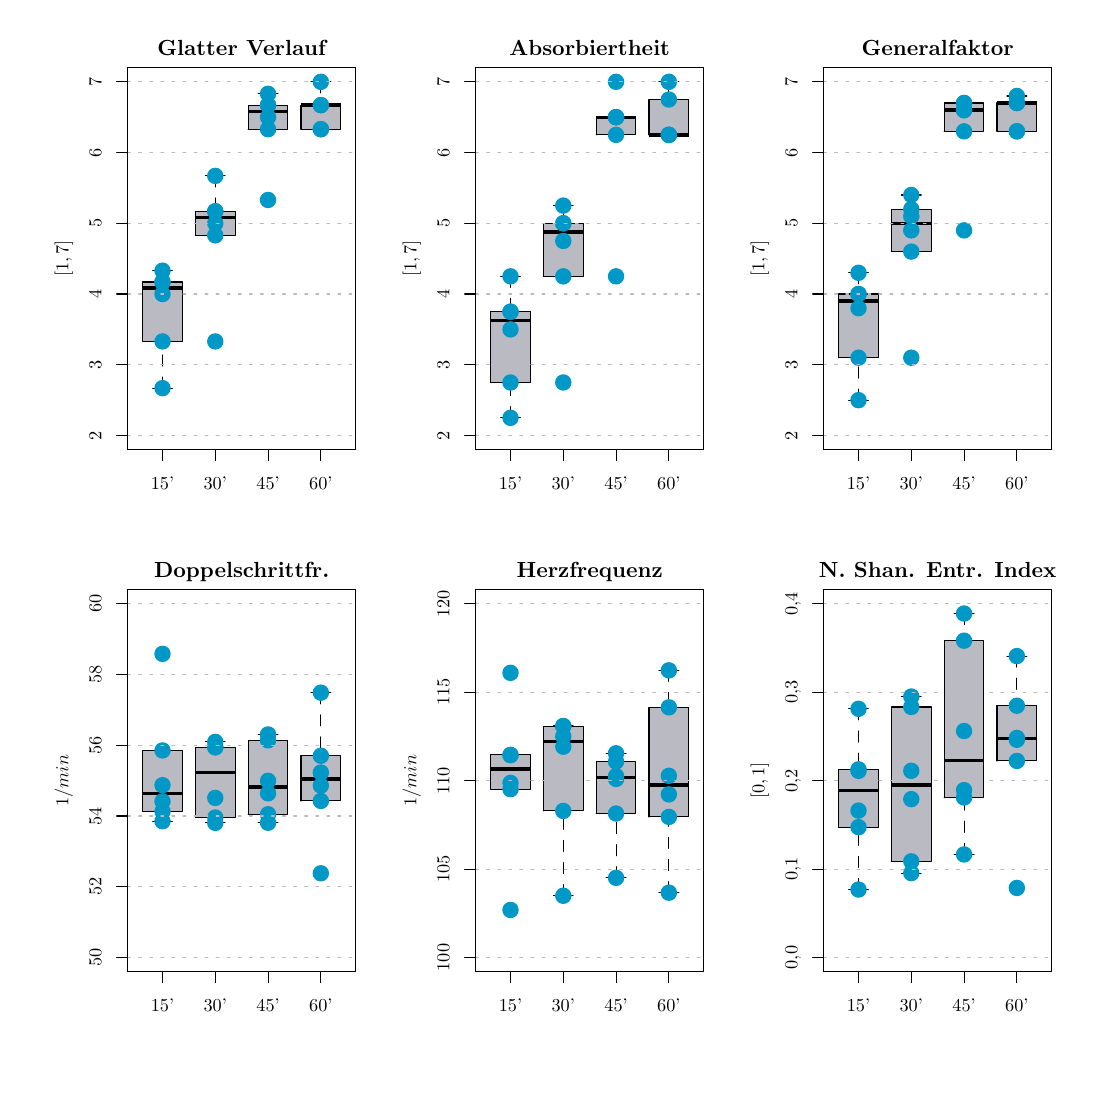
\begin{tikzpicture}[x=1pt,y=1pt]
\definecolor{fillColor}{RGB}{255,255,255}
\path[use as bounding box,fill=fillColor] (0,0) rectangle (377.25,377.25);
\begin{scope}
\path[clip] ( 36.13,224.76) rectangle (118.52,362.80);
\definecolor{fillColor}{RGB}{186,187,194}

\path[fill=fillColor] ( 41.57,263.87) --
	( 55.87,263.87) --
	( 55.87,285.34) --
	( 41.57,285.34) --
	cycle;
\definecolor{drawColor}{RGB}{0,0,0}

\path[draw=drawColor,line width= 1.2pt,line join=round] ( 41.57,283.17) -- ( 55.87,283.17);

\path[draw=drawColor,line width= 0.4pt,dash pattern=on 4pt off 4pt ,line join=round,line cap=round] ( 48.72,247.00) -- ( 48.72,263.87);

\path[draw=drawColor,line width= 0.4pt,dash pattern=on 4pt off 4pt ,line join=round,line cap=round] ( 48.72,289.43) -- ( 48.72,285.34);

\path[draw=drawColor,line width= 0.4pt,line join=round,line cap=round] ( 45.15,247.00) -- ( 52.30,247.00);

\path[draw=drawColor,line width= 0.4pt,line join=round,line cap=round] ( 45.15,289.43) -- ( 52.30,289.43);

\path[draw=drawColor,line width= 0.4pt,line join=round,line cap=round] ( 41.57,263.87) --
	( 55.87,263.87) --
	( 55.87,285.34) --
	( 41.57,285.34) --
	( 41.57,263.87);

\path[fill=fillColor] ( 60.64,302.21) --
	( 74.94,302.21) --
	( 74.94,310.90) --
	( 60.64,310.90) --
	cycle;

\path[draw=drawColor,line width= 1.2pt,line join=round] ( 60.64,308.73) -- ( 74.94,308.73);

\path[draw=drawColor,line width= 0.4pt,dash pattern=on 4pt off 4pt ,line join=round,line cap=round] ( 67.79,302.21) -- ( 67.79,302.21);

\path[draw=drawColor,line width= 0.4pt,dash pattern=on 4pt off 4pt ,line join=round,line cap=round] ( 67.79,323.69) -- ( 67.79,310.90);

\path[draw=drawColor,line width= 0.4pt,line join=round,line cap=round] ( 64.22,302.21) -- ( 71.37,302.21);

\path[draw=drawColor,line width= 0.4pt,line join=round,line cap=round] ( 64.22,323.69) -- ( 71.37,323.69);

\path[draw=drawColor,line width= 0.4pt,line join=round,line cap=round] ( 60.64,302.21) --
	( 74.94,302.21) --
	( 74.94,310.90) --
	( 60.64,310.90) --
	( 60.64,302.21);

\path[fill=fillColor] ( 79.71,340.56) --
	( 94.02,340.56) --
	( 94.02,349.25) --
	( 79.71,349.25) --
	cycle;

\path[draw=drawColor,line width= 1.2pt,line join=round] ( 79.71,347.07) -- ( 94.02,347.07);

\path[draw=drawColor,line width= 0.4pt,dash pattern=on 4pt off 4pt ,line join=round,line cap=round] ( 86.86,340.56) -- ( 86.86,340.56);

\path[draw=drawColor,line width= 0.4pt,dash pattern=on 4pt off 4pt ,line join=round,line cap=round] ( 86.86,353.34) -- ( 86.86,349.25);

\path[draw=drawColor,line width= 0.4pt,line join=round,line cap=round] ( 83.29,340.56) -- ( 90.44,340.56);

\path[draw=drawColor,line width= 0.4pt,line join=round,line cap=round] ( 83.29,353.34) -- ( 90.44,353.34);

\path[draw=drawColor,line width= 0.4pt,line join=round,line cap=round] ( 79.71,340.56) --
	( 94.02,340.56) --
	( 94.02,349.25) --
	( 79.71,349.25) --
	( 79.71,340.56);

\path[fill=fillColor] ( 98.78,340.56) --
	(113.09,340.56) --
	(113.09,349.25) --
	( 98.78,349.25) --
	cycle;

\path[draw=drawColor,line width= 1.2pt,line join=round] ( 98.78,349.25) -- (113.09,349.25);

\path[draw=drawColor,line width= 0.4pt,dash pattern=on 4pt off 4pt ,line join=round,line cap=round] (105.94,340.56) -- (105.94,340.56);

\path[draw=drawColor,line width= 0.4pt,dash pattern=on 4pt off 4pt ,line join=round,line cap=round] (105.94,357.68) -- (105.94,349.25);

\path[draw=drawColor,line width= 0.4pt,line join=round,line cap=round] (102.36,340.56) -- (109.51,340.56);

\path[draw=drawColor,line width= 0.4pt,line join=round,line cap=round] (102.36,357.68) -- (109.51,357.68);

\path[draw=drawColor,line width= 0.4pt,line join=round,line cap=round] ( 98.78,340.56) --
	(113.09,340.56) --
	(113.09,349.25) --
	( 98.78,349.25) --
	( 98.78,340.56);
\end{scope}
\begin{scope}
\path[clip] (  0.00,  0.00) rectangle (377.25,377.25);
\definecolor{drawColor}{RGB}{0,0,0}

\path[draw=drawColor,line width= 0.4pt,line join=round,line cap=round] ( 48.72,224.76) -- (105.94,224.76);

\path[draw=drawColor,line width= 0.4pt,line join=round,line cap=round] ( 48.72,224.76) -- ( 48.72,220.80);

\path[draw=drawColor,line width= 0.4pt,line join=round,line cap=round] ( 67.79,224.76) -- ( 67.79,220.80);

\path[draw=drawColor,line width= 0.4pt,line join=round,line cap=round] ( 86.86,224.76) -- ( 86.86,220.80);

\path[draw=drawColor,line width= 0.4pt,line join=round,line cap=round] (105.94,224.76) -- (105.94,220.80);

\node[text=drawColor,anchor=base,inner sep=0pt, outer sep=0pt, scale=  0.66] at ( 48.72,210.50) {15'};

\node[text=drawColor,anchor=base,inner sep=0pt, outer sep=0pt, scale=  0.66] at ( 67.79,210.50) {30'};

\node[text=drawColor,anchor=base,inner sep=0pt, outer sep=0pt, scale=  0.66] at ( 86.86,210.50) {45'};

\node[text=drawColor,anchor=base,inner sep=0pt, outer sep=0pt, scale=  0.66] at (105.94,210.50) {60'};

\path[draw=drawColor,line width= 0.4pt,line join=round,line cap=round] ( 36.13,229.87) -- ( 36.13,357.68);

\path[draw=drawColor,line width= 0.4pt,line join=round,line cap=round] ( 36.13,229.87) -- ( 32.17,229.87);

\path[draw=drawColor,line width= 0.4pt,line join=round,line cap=round] ( 36.13,255.43) -- ( 32.17,255.43);

\path[draw=drawColor,line width= 0.4pt,line join=round,line cap=round] ( 36.13,281.00) -- ( 32.17,281.00);

\path[draw=drawColor,line width= 0.4pt,line join=round,line cap=round] ( 36.13,306.56) -- ( 32.17,306.56);

\path[draw=drawColor,line width= 0.4pt,line join=round,line cap=round] ( 36.13,332.12) -- ( 32.17,332.12);

\path[draw=drawColor,line width= 0.4pt,line join=round,line cap=round] ( 36.13,357.68) -- ( 32.17,357.68);

\node[text=drawColor,rotate= 90.00,anchor=base,inner sep=0pt, outer sep=0pt, scale=  0.66] at ( 26.63,229.87) {2};

\node[text=drawColor,rotate= 90.00,anchor=base,inner sep=0pt, outer sep=0pt, scale=  0.66] at ( 26.63,255.43) {3};

\node[text=drawColor,rotate= 90.00,anchor=base,inner sep=0pt, outer sep=0pt, scale=  0.66] at ( 26.63,281.00) {4};

\node[text=drawColor,rotate= 90.00,anchor=base,inner sep=0pt, outer sep=0pt, scale=  0.66] at ( 26.63,306.56) {5};

\node[text=drawColor,rotate= 90.00,anchor=base,inner sep=0pt, outer sep=0pt, scale=  0.66] at ( 26.63,332.12) {6};

\node[text=drawColor,rotate= 90.00,anchor=base,inner sep=0pt, outer sep=0pt, scale=  0.66] at ( 26.63,357.68) {7};
\end{scope}
\begin{scope}
\path[clip] (  0.00,188.62) rectangle (125.75,377.25);
\definecolor{drawColor}{RGB}{0,0,0}

\node[text=drawColor,anchor=base,inner sep=0pt, outer sep=0pt, scale=  0.79] at ( 77.33,367.29) {\bfseries Glatter Verlauf};

\node[text=drawColor,rotate= 90.00,anchor=base,inner sep=0pt, outer sep=0pt, scale=  0.66] at ( 14.75,293.78) {$[1, 7]$};
\end{scope}
\begin{scope}
\path[clip] (  0.00,  0.00) rectangle (377.25,377.25);
\definecolor{drawColor}{RGB}{0,0,0}

\path[draw=drawColor,line width= 0.4pt,line join=round,line cap=round] ( 36.13,224.76) --
	(118.52,224.76) --
	(118.52,362.80) --
	( 36.13,362.80) --
	( 36.13,224.76);
\end{scope}
\begin{scope}
\path[clip] ( 36.13,224.76) rectangle (118.52,362.80);
\definecolor{fillColor}{RGB}{0,152,199}

\path[fill=fillColor] ( 48.72,247.00) circle (  2.97);

\path[fill=fillColor] ( 67.79,263.87) circle (  2.97);

\path[fill=fillColor] ( 86.86,314.99) circle (  2.97);

\path[fill=fillColor] (105.94,340.56) circle (  2.97);

\path[fill=fillColor] ( 48.72,263.87) circle (  2.97);

\path[fill=fillColor] ( 67.79,302.21) circle (  2.97);

\path[fill=fillColor] ( 86.86,340.56) circle (  2.97);

\path[fill=fillColor] (105.94,340.56) circle (  2.97);

\path[fill=fillColor] ( 48.72,285.34) circle (  2.97);

\path[fill=fillColor] ( 67.79,323.69) circle (  2.97);

\path[fill=fillColor] ( 86.86,349.25) circle (  2.97);

\path[fill=fillColor] ( 48.72,289.43) circle (  2.97);

\path[fill=fillColor] ( 67.79,310.90) circle (  2.97);

\path[fill=fillColor] ( 86.86,349.25) circle (  2.97);

\path[fill=fillColor] (105.94,349.25) circle (  2.97);

\path[fill=fillColor] ( 48.72,285.34) circle (  2.97);

\path[fill=fillColor] ( 67.79,306.56) circle (  2.97);

\path[fill=fillColor] ( 86.86,353.34) circle (  2.97);

\path[fill=fillColor] (105.94,349.25) circle (  2.97);

\path[fill=fillColor] ( 48.72,281.00) circle (  2.97);

\path[fill=fillColor] ( 67.79,310.90) circle (  2.97);

\path[fill=fillColor] ( 86.86,344.90) circle (  2.97);

\path[fill=fillColor] (105.94,357.68) circle (  2.97);
\definecolor{drawColor}{RGB}{186,187,194}

\path[draw=drawColor,line width= 0.4pt,dash pattern=on 1pt off 3pt ,line join=round,line cap=round] ( 36.13,229.87) -- (118.52,229.87);

\path[draw=drawColor,line width= 0.4pt,dash pattern=on 1pt off 3pt ,line join=round,line cap=round] ( 36.13,255.43) -- (118.52,255.43);

\path[draw=drawColor,line width= 0.4pt,dash pattern=on 1pt off 3pt ,line join=round,line cap=round] ( 36.13,281.00) -- (118.52,281.00);

\path[draw=drawColor,line width= 0.4pt,dash pattern=on 1pt off 3pt ,line join=round,line cap=round] ( 36.13,306.56) -- (118.52,306.56);

\path[draw=drawColor,line width= 0.4pt,dash pattern=on 1pt off 3pt ,line join=round,line cap=round] ( 36.13,332.12) -- (118.52,332.12);

\path[draw=drawColor,line width= 0.4pt,dash pattern=on 1pt off 3pt ,line join=round,line cap=round] ( 36.13,357.68) -- (118.52,357.68);
\end{scope}
\begin{scope}
\path[clip] (  0.00,  0.00) rectangle (377.25,377.25);
\definecolor{drawColor}{RGB}{0,0,0}

\path[draw=drawColor,line width= 0.4pt,line join=round,line cap=round] ( 36.13,224.76) --
	(118.52,224.76) --
	(118.52,362.80) --
	( 36.13,362.80) --
	( 36.13,224.76);
\end{scope}
\begin{scope}
\path[clip] (161.88,224.76) rectangle (244.27,362.80);
\definecolor{fillColor}{RGB}{186,187,194}

\path[fill=fillColor] (167.32,249.04) --
	(181.62,249.04) --
	(181.62,274.61) --
	(167.32,274.61) --
	cycle;
\definecolor{drawColor}{RGB}{0,0,0}

\path[draw=drawColor,line width= 1.2pt,line join=round] (167.32,271.41) -- (181.62,271.41);

\path[draw=drawColor,line width= 0.4pt,dash pattern=on 4pt off 4pt ,line join=round,line cap=round] (174.47,236.26) -- (174.47,249.04);

\path[draw=drawColor,line width= 0.4pt,dash pattern=on 4pt off 4pt ,line join=round,line cap=round] (174.47,287.39) -- (174.47,274.61);

\path[draw=drawColor,line width= 0.4pt,line join=round,line cap=round] (170.90,236.26) -- (178.05,236.26);

\path[draw=drawColor,line width= 0.4pt,line join=round,line cap=round] (170.90,287.39) -- (178.05,287.39);

\path[draw=drawColor,line width= 0.4pt,line join=round,line cap=round] (167.32,249.04) --
	(181.62,249.04) --
	(181.62,274.61) --
	(167.32,274.61) --
	(167.32,249.04);

\path[fill=fillColor] (186.39,287.39) --
	(200.69,287.39) --
	(200.69,306.56) --
	(186.39,306.56) --
	cycle;

\path[draw=drawColor,line width= 1.2pt,line join=round] (186.39,303.36) -- (200.69,303.36);

\path[draw=drawColor,line width= 0.4pt,dash pattern=on 4pt off 4pt ,line join=round,line cap=round] (193.54,287.39) -- (193.54,287.39);

\path[draw=drawColor,line width= 0.4pt,dash pattern=on 4pt off 4pt ,line join=round,line cap=round] (193.54,312.95) -- (193.54,306.56);

\path[draw=drawColor,line width= 0.4pt,line join=round,line cap=round] (189.97,287.39) -- (197.12,287.39);

\path[draw=drawColor,line width= 0.4pt,line join=round,line cap=round] (189.97,312.95) -- (197.12,312.95);

\path[draw=drawColor,line width= 0.4pt,line join=round,line cap=round] (186.39,287.39) --
	(200.69,287.39) --
	(200.69,306.56) --
	(186.39,306.56) --
	(186.39,287.39);

\path[fill=fillColor] (205.46,338.51) --
	(219.77,338.51) --
	(219.77,344.90) --
	(205.46,344.90) --
	cycle;

\path[draw=drawColor,line width= 1.2pt,line join=round] (205.46,344.90) -- (219.77,344.90);

\path[draw=drawColor,line width= 0.4pt,dash pattern=on 4pt off 4pt ,line join=round,line cap=round] (212.61,338.51) -- (212.61,338.51);

\path[draw=drawColor,line width= 0.4pt,dash pattern=on 4pt off 4pt ,line join=round,line cap=round] (212.61,344.90) -- (212.61,344.90);

\path[draw=drawColor,line width= 0.4pt,line join=round,line cap=round] (209.04,338.51) -- (216.19,338.51);

\path[draw=drawColor,line width= 0.4pt,line join=round,line cap=round] (209.04,344.90) -- (216.19,344.90);

\path[draw=drawColor,line width= 0.4pt,line join=round,line cap=round] (205.46,338.51) --
	(219.77,338.51) --
	(219.77,344.90) --
	(205.46,344.90) --
	(205.46,338.51);

\path[fill=fillColor] (224.53,338.51) --
	(238.84,338.51) --
	(238.84,351.29) --
	(224.53,351.29) --
	cycle;

\path[draw=drawColor,line width= 1.2pt,line join=round] (224.53,338.51) -- (238.84,338.51);

\path[draw=drawColor,line width= 0.4pt,dash pattern=on 4pt off 4pt ,line join=round,line cap=round] (231.69,338.51) -- (231.69,338.51);

\path[draw=drawColor,line width= 0.4pt,dash pattern=on 4pt off 4pt ,line join=round,line cap=round] (231.69,357.68) -- (231.69,351.29);

\path[draw=drawColor,line width= 0.4pt,line join=round,line cap=round] (228.11,338.51) -- (235.26,338.51);

\path[draw=drawColor,line width= 0.4pt,line join=round,line cap=round] (228.11,357.68) -- (235.26,357.68);

\path[draw=drawColor,line width= 0.4pt,line join=round,line cap=round] (224.53,338.51) --
	(238.84,338.51) --
	(238.84,351.29) --
	(224.53,351.29) --
	(224.53,338.51);
\end{scope}
\begin{scope}
\path[clip] (  0.00,  0.00) rectangle (377.25,377.25);
\definecolor{drawColor}{RGB}{0,0,0}

\path[draw=drawColor,line width= 0.4pt,line join=round,line cap=round] (174.47,224.76) -- (231.69,224.76);

\path[draw=drawColor,line width= 0.4pt,line join=round,line cap=round] (174.47,224.76) -- (174.47,220.80);

\path[draw=drawColor,line width= 0.4pt,line join=round,line cap=round] (193.54,224.76) -- (193.54,220.80);

\path[draw=drawColor,line width= 0.4pt,line join=round,line cap=round] (212.61,224.76) -- (212.61,220.80);

\path[draw=drawColor,line width= 0.4pt,line join=round,line cap=round] (231.69,224.76) -- (231.69,220.80);

\node[text=drawColor,anchor=base,inner sep=0pt, outer sep=0pt, scale=  0.66] at (174.47,210.50) {15'};

\node[text=drawColor,anchor=base,inner sep=0pt, outer sep=0pt, scale=  0.66] at (193.54,210.50) {30'};

\node[text=drawColor,anchor=base,inner sep=0pt, outer sep=0pt, scale=  0.66] at (212.61,210.50) {45'};

\node[text=drawColor,anchor=base,inner sep=0pt, outer sep=0pt, scale=  0.66] at (231.69,210.50) {60'};

\path[draw=drawColor,line width= 0.4pt,line join=round,line cap=round] (161.88,229.87) -- (161.88,357.68);

\path[draw=drawColor,line width= 0.4pt,line join=round,line cap=round] (161.88,229.87) -- (157.92,229.87);

\path[draw=drawColor,line width= 0.4pt,line join=round,line cap=round] (161.88,255.43) -- (157.92,255.43);

\path[draw=drawColor,line width= 0.4pt,line join=round,line cap=round] (161.88,281.00) -- (157.92,281.00);

\path[draw=drawColor,line width= 0.4pt,line join=round,line cap=round] (161.88,306.56) -- (157.92,306.56);

\path[draw=drawColor,line width= 0.4pt,line join=round,line cap=round] (161.88,332.12) -- (157.92,332.12);

\path[draw=drawColor,line width= 0.4pt,line join=round,line cap=round] (161.88,357.68) -- (157.92,357.68);

\node[text=drawColor,rotate= 90.00,anchor=base,inner sep=0pt, outer sep=0pt, scale=  0.66] at (152.38,229.87) {2};

\node[text=drawColor,rotate= 90.00,anchor=base,inner sep=0pt, outer sep=0pt, scale=  0.66] at (152.38,255.43) {3};

\node[text=drawColor,rotate= 90.00,anchor=base,inner sep=0pt, outer sep=0pt, scale=  0.66] at (152.38,281.00) {4};

\node[text=drawColor,rotate= 90.00,anchor=base,inner sep=0pt, outer sep=0pt, scale=  0.66] at (152.38,306.56) {5};

\node[text=drawColor,rotate= 90.00,anchor=base,inner sep=0pt, outer sep=0pt, scale=  0.66] at (152.38,332.12) {6};

\node[text=drawColor,rotate= 90.00,anchor=base,inner sep=0pt, outer sep=0pt, scale=  0.66] at (152.38,357.68) {7};
\end{scope}
\begin{scope}
\path[clip] (125.75,188.62) rectangle (251.50,377.25);
\definecolor{drawColor}{RGB}{0,0,0}

\node[text=drawColor,anchor=base,inner sep=0pt, outer sep=0pt, scale=  0.79] at (203.08,367.29) {\bfseries Absorbiertheit};

\node[text=drawColor,rotate= 90.00,anchor=base,inner sep=0pt, outer sep=0pt, scale=  0.66] at (140.50,293.78) {$[1, 7]$};
\end{scope}
\begin{scope}
\path[clip] (  0.00,  0.00) rectangle (377.25,377.25);
\definecolor{drawColor}{RGB}{0,0,0}

\path[draw=drawColor,line width= 0.4pt,line join=round,line cap=round] (161.88,224.76) --
	(244.27,224.76) --
	(244.27,362.80) --
	(161.88,362.80) --
	(161.88,224.76);
\end{scope}
\begin{scope}
\path[clip] (161.88,224.76) rectangle (244.27,362.80);
\definecolor{fillColor}{RGB}{0,152,199}

\path[fill=fillColor] (174.47,236.26) circle (  2.97);

\path[fill=fillColor] (193.54,249.04) circle (  2.97);

\path[fill=fillColor] (212.61,287.39) circle (  2.97);

\path[fill=fillColor] (231.69,338.51) circle (  2.97);

\path[fill=fillColor] (174.47,249.04) circle (  2.97);

\path[fill=fillColor] (193.54,287.39) circle (  2.97);

\path[fill=fillColor] (212.61,338.51) circle (  2.97);

\path[fill=fillColor] (231.69,338.51) circle (  2.97);

\path[fill=fillColor] (174.47,274.61) circle (  2.97);

\path[fill=fillColor] (193.54,306.56) circle (  2.97);

\path[fill=fillColor] (212.61,344.90) circle (  2.97);

\path[fill=fillColor] (174.47,287.39) circle (  2.97);

\path[fill=fillColor] (193.54,312.95) circle (  2.97);

\path[fill=fillColor] (212.61,344.90) circle (  2.97);

\path[fill=fillColor] (231.69,351.29) circle (  2.97);

\path[fill=fillColor] (174.47,274.61) circle (  2.97);

\path[fill=fillColor] (193.54,300.17) circle (  2.97);

\path[fill=fillColor] (212.61,344.90) circle (  2.97);

\path[fill=fillColor] (231.69,357.68) circle (  2.97);

\path[fill=fillColor] (174.47,268.22) circle (  2.97);

\path[fill=fillColor] (193.54,306.56) circle (  2.97);

\path[fill=fillColor] (212.61,357.68) circle (  2.97);

\path[fill=fillColor] (231.69,338.51) circle (  2.97);
\definecolor{drawColor}{RGB}{186,187,194}

\path[draw=drawColor,line width= 0.4pt,dash pattern=on 1pt off 3pt ,line join=round,line cap=round] (161.88,229.87) -- (244.27,229.87);

\path[draw=drawColor,line width= 0.4pt,dash pattern=on 1pt off 3pt ,line join=round,line cap=round] (161.88,255.43) -- (244.27,255.43);

\path[draw=drawColor,line width= 0.4pt,dash pattern=on 1pt off 3pt ,line join=round,line cap=round] (161.88,281.00) -- (244.27,281.00);

\path[draw=drawColor,line width= 0.4pt,dash pattern=on 1pt off 3pt ,line join=round,line cap=round] (161.88,306.56) -- (244.27,306.56);

\path[draw=drawColor,line width= 0.4pt,dash pattern=on 1pt off 3pt ,line join=round,line cap=round] (161.88,332.12) -- (244.27,332.12);

\path[draw=drawColor,line width= 0.4pt,dash pattern=on 1pt off 3pt ,line join=round,line cap=round] (161.88,357.68) -- (244.27,357.68);
\end{scope}
\begin{scope}
\path[clip] (  0.00,  0.00) rectangle (377.25,377.25);
\definecolor{drawColor}{RGB}{0,0,0}

\path[draw=drawColor,line width= 0.4pt,line join=round,line cap=round] (161.88,224.76) --
	(244.27,224.76) --
	(244.27,362.80) --
	(161.88,362.80) --
	(161.88,224.76);
\end{scope}
\begin{scope}
\path[clip] (287.63,224.76) rectangle (370.02,362.80);
\definecolor{fillColor}{RGB}{186,187,194}

\path[fill=fillColor] (293.07,257.99) --
	(307.37,257.99) --
	(307.37,281.00) --
	(293.07,281.00) --
	cycle;
\definecolor{drawColor}{RGB}{0,0,0}

\path[draw=drawColor,line width= 1.2pt,line join=round] (293.07,278.44) -- (307.37,278.44);

\path[draw=drawColor,line width= 0.4pt,dash pattern=on 4pt off 4pt ,line join=round,line cap=round] (300.22,242.65) -- (300.22,257.99);

\path[draw=drawColor,line width= 0.4pt,dash pattern=on 4pt off 4pt ,line join=round,line cap=round] (300.22,288.67) -- (300.22,281.00);

\path[draw=drawColor,line width= 0.4pt,line join=round,line cap=round] (296.65,242.65) -- (303.80,242.65);

\path[draw=drawColor,line width= 0.4pt,line join=round,line cap=round] (296.65,288.67) -- (303.80,288.67);

\path[draw=drawColor,line width= 0.4pt,line join=round,line cap=round] (293.07,257.99) --
	(307.37,257.99) --
	(307.37,281.00) --
	(293.07,281.00) --
	(293.07,257.99);

\path[fill=fillColor] (312.14,296.33) --
	(326.44,296.33) --
	(326.44,311.67) --
	(312.14,311.67) --
	cycle;

\path[draw=drawColor,line width= 1.2pt,line join=round] (312.14,306.56) -- (326.44,306.56);

\path[draw=drawColor,line width= 0.4pt,dash pattern=on 4pt off 4pt ,line join=round,line cap=round] (319.29,296.33) -- (319.29,296.33);

\path[draw=drawColor,line width= 0.4pt,dash pattern=on 4pt off 4pt ,line join=round,line cap=round] (319.29,316.78) -- (319.29,311.67);

\path[draw=drawColor,line width= 0.4pt,line join=round,line cap=round] (315.72,296.33) -- (322.87,296.33);

\path[draw=drawColor,line width= 0.4pt,line join=round,line cap=round] (315.72,316.78) -- (322.87,316.78);

\path[draw=drawColor,line width= 0.4pt,line join=round,line cap=round] (312.14,296.33) --
	(326.44,296.33) --
	(326.44,311.67) --
	(312.14,311.67) --
	(312.14,296.33);

\path[fill=fillColor] (331.21,339.79) --
	(345.52,339.79) --
	(345.52,350.01) --
	(331.21,350.01) --
	cycle;

\path[draw=drawColor,line width= 1.2pt,line join=round] (331.21,347.46) -- (345.52,347.46);

\path[draw=drawColor,line width= 0.4pt,dash pattern=on 4pt off 4pt ,line join=round,line cap=round] (338.36,339.79) -- (338.36,339.79);

\path[draw=drawColor,line width= 0.4pt,dash pattern=on 4pt off 4pt ,line join=round,line cap=round] (338.36,350.01) -- (338.36,350.01);

\path[draw=drawColor,line width= 0.4pt,line join=round,line cap=round] (334.79,339.79) -- (341.94,339.79);

\path[draw=drawColor,line width= 0.4pt,line join=round,line cap=round] (334.79,350.01) -- (341.94,350.01);

\path[draw=drawColor,line width= 0.4pt,line join=round,line cap=round] (331.21,339.79) --
	(345.52,339.79) --
	(345.52,350.01) --
	(331.21,350.01) --
	(331.21,339.79);

\path[fill=fillColor] (350.28,339.79) --
	(364.59,339.79) --
	(364.59,350.01) --
	(350.28,350.01) --
	cycle;

\path[draw=drawColor,line width= 1.2pt,line join=round] (350.28,350.01) -- (364.59,350.01);

\path[draw=drawColor,line width= 0.4pt,dash pattern=on 4pt off 4pt ,line join=round,line cap=round] (357.44,339.79) -- (357.44,339.79);

\path[draw=drawColor,line width= 0.4pt,dash pattern=on 4pt off 4pt ,line join=round,line cap=round] (357.44,352.57) -- (357.44,350.01);

\path[draw=drawColor,line width= 0.4pt,line join=round,line cap=round] (353.86,339.79) -- (361.01,339.79);

\path[draw=drawColor,line width= 0.4pt,line join=round,line cap=round] (353.86,352.57) -- (361.01,352.57);

\path[draw=drawColor,line width= 0.4pt,line join=round,line cap=round] (350.28,339.79) --
	(364.59,339.79) --
	(364.59,350.01) --
	(350.28,350.01) --
	(350.28,339.79);
\end{scope}
\begin{scope}
\path[clip] (  0.00,  0.00) rectangle (377.25,377.25);
\definecolor{drawColor}{RGB}{0,0,0}

\path[draw=drawColor,line width= 0.4pt,line join=round,line cap=round] (300.22,224.76) -- (357.44,224.76);

\path[draw=drawColor,line width= 0.4pt,line join=round,line cap=round] (300.22,224.76) -- (300.22,220.80);

\path[draw=drawColor,line width= 0.4pt,line join=round,line cap=round] (319.29,224.76) -- (319.29,220.80);

\path[draw=drawColor,line width= 0.4pt,line join=round,line cap=round] (338.36,224.76) -- (338.36,220.80);

\path[draw=drawColor,line width= 0.4pt,line join=round,line cap=round] (357.44,224.76) -- (357.44,220.80);

\node[text=drawColor,anchor=base,inner sep=0pt, outer sep=0pt, scale=  0.66] at (300.22,210.50) {15'};

\node[text=drawColor,anchor=base,inner sep=0pt, outer sep=0pt, scale=  0.66] at (319.29,210.50) {30'};

\node[text=drawColor,anchor=base,inner sep=0pt, outer sep=0pt, scale=  0.66] at (338.36,210.50) {45'};

\node[text=drawColor,anchor=base,inner sep=0pt, outer sep=0pt, scale=  0.66] at (357.44,210.50) {60'};

\path[draw=drawColor,line width= 0.4pt,line join=round,line cap=round] (287.63,229.87) -- (287.63,357.68);

\path[draw=drawColor,line width= 0.4pt,line join=round,line cap=round] (287.63,229.87) -- (283.67,229.87);

\path[draw=drawColor,line width= 0.4pt,line join=round,line cap=round] (287.63,255.43) -- (283.67,255.43);

\path[draw=drawColor,line width= 0.4pt,line join=round,line cap=round] (287.63,281.00) -- (283.67,281.00);

\path[draw=drawColor,line width= 0.4pt,line join=round,line cap=round] (287.63,306.56) -- (283.67,306.56);

\path[draw=drawColor,line width= 0.4pt,line join=round,line cap=round] (287.63,332.12) -- (283.67,332.12);

\path[draw=drawColor,line width= 0.4pt,line join=round,line cap=round] (287.63,357.68) -- (283.67,357.68);

\node[text=drawColor,rotate= 90.00,anchor=base,inner sep=0pt, outer sep=0pt, scale=  0.66] at (278.13,229.87) {2};

\node[text=drawColor,rotate= 90.00,anchor=base,inner sep=0pt, outer sep=0pt, scale=  0.66] at (278.13,255.43) {3};

\node[text=drawColor,rotate= 90.00,anchor=base,inner sep=0pt, outer sep=0pt, scale=  0.66] at (278.13,281.00) {4};

\node[text=drawColor,rotate= 90.00,anchor=base,inner sep=0pt, outer sep=0pt, scale=  0.66] at (278.13,306.56) {5};

\node[text=drawColor,rotate= 90.00,anchor=base,inner sep=0pt, outer sep=0pt, scale=  0.66] at (278.13,332.12) {6};

\node[text=drawColor,rotate= 90.00,anchor=base,inner sep=0pt, outer sep=0pt, scale=  0.66] at (278.13,357.68) {7};
\end{scope}
\begin{scope}
\path[clip] (251.50,188.62) rectangle (377.25,377.25);
\definecolor{drawColor}{RGB}{0,0,0}

\node[text=drawColor,anchor=base,inner sep=0pt, outer sep=0pt, scale=  0.79] at (328.83,367.29) {\bfseries Generalfaktor};

\node[text=drawColor,rotate= 90.00,anchor=base,inner sep=0pt, outer sep=0pt, scale=  0.66] at (266.25,293.78) {$[1, 7]$};
\end{scope}
\begin{scope}
\path[clip] (  0.00,  0.00) rectangle (377.25,377.25);
\definecolor{drawColor}{RGB}{0,0,0}

\path[draw=drawColor,line width= 0.4pt,line join=round,line cap=round] (287.63,224.76) --
	(370.02,224.76) --
	(370.02,362.80) --
	(287.63,362.80) --
	(287.63,224.76);
\end{scope}
\begin{scope}
\path[clip] (287.63,224.76) rectangle (370.02,362.80);
\definecolor{fillColor}{RGB}{0,152,199}

\path[fill=fillColor] (300.22,242.65) circle (  2.97);

\path[fill=fillColor] (319.29,257.99) circle (  2.97);

\path[fill=fillColor] (338.36,304.00) circle (  2.97);

\path[fill=fillColor] (357.44,339.79) circle (  2.97);

\path[fill=fillColor] (300.22,257.99) circle (  2.97);

\path[fill=fillColor] (319.29,296.33) circle (  2.97);

\path[fill=fillColor] (338.36,339.79) circle (  2.97);

\path[fill=fillColor] (357.44,339.79) circle (  2.97);

\path[fill=fillColor] (300.22,281.00) circle (  2.97);

\path[fill=fillColor] (319.29,316.78) circle (  2.97);

\path[fill=fillColor] (338.36,347.46) circle (  2.97);

\path[fill=fillColor] (300.22,288.67) circle (  2.97);

\path[fill=fillColor] (319.29,311.67) circle (  2.97);

\path[fill=fillColor] (338.36,347.46) circle (  2.97);

\path[fill=fillColor] (357.44,350.01) circle (  2.97);

\path[fill=fillColor] (300.22,281.00) circle (  2.97);

\path[fill=fillColor] (319.29,304.00) circle (  2.97);

\path[fill=fillColor] (338.36,350.01) circle (  2.97);

\path[fill=fillColor] (357.44,352.57) circle (  2.97);

\path[fill=fillColor] (300.22,275.88) circle (  2.97);

\path[fill=fillColor] (319.29,309.11) circle (  2.97);

\path[fill=fillColor] (338.36,350.01) circle (  2.97);

\path[fill=fillColor] (357.44,350.01) circle (  2.97);
\definecolor{drawColor}{RGB}{186,187,194}

\path[draw=drawColor,line width= 0.4pt,dash pattern=on 1pt off 3pt ,line join=round,line cap=round] (287.63,229.87) -- (370.02,229.87);

\path[draw=drawColor,line width= 0.4pt,dash pattern=on 1pt off 3pt ,line join=round,line cap=round] (287.63,255.43) -- (370.02,255.43);

\path[draw=drawColor,line width= 0.4pt,dash pattern=on 1pt off 3pt ,line join=round,line cap=round] (287.63,281.00) -- (370.02,281.00);

\path[draw=drawColor,line width= 0.4pt,dash pattern=on 1pt off 3pt ,line join=round,line cap=round] (287.63,306.56) -- (370.02,306.56);

\path[draw=drawColor,line width= 0.4pt,dash pattern=on 1pt off 3pt ,line join=round,line cap=round] (287.63,332.12) -- (370.02,332.12);

\path[draw=drawColor,line width= 0.4pt,dash pattern=on 1pt off 3pt ,line join=round,line cap=round] (287.63,357.68) -- (370.02,357.68);
\end{scope}
\begin{scope}
\path[clip] (  0.00,  0.00) rectangle (377.25,377.25);
\definecolor{drawColor}{RGB}{0,0,0}

\path[draw=drawColor,line width= 0.4pt,line join=round,line cap=round] (287.63,224.76) --
	(370.02,224.76) --
	(370.02,362.80) --
	(287.63,362.80) --
	(287.63,224.76);
\end{scope}
\begin{scope}
\path[clip] ( 36.13, 36.13) rectangle (118.52,174.17);
\definecolor{fillColor}{RGB}{186,187,194}

\path[fill=fillColor] ( 41.57, 94.06) --
	( 55.87, 94.06) --
	( 55.87,116.08) --
	( 41.57,116.08) --
	cycle;
\definecolor{drawColor}{RGB}{0,0,0}

\path[draw=drawColor,line width= 1.2pt,line join=round] ( 41.57,100.60) -- ( 55.87,100.60);

\path[draw=drawColor,line width= 0.4pt,dash pattern=on 4pt off 4pt ,line join=round,line cap=round] ( 48.72, 90.50) -- ( 48.72, 94.06);

\path[draw=drawColor,line width= 0.4pt,dash pattern=on 4pt off 4pt ,line join=round,line cap=round] ( 48.72,116.08) -- ( 48.72,116.08);

\path[draw=drawColor,line width= 0.4pt,line join=round,line cap=round] ( 45.15, 90.50) -- ( 52.30, 90.50);

\path[draw=drawColor,line width= 0.4pt,line join=round,line cap=round] ( 45.15,116.08) -- ( 52.30,116.08);

\path[draw=drawColor,line width= 0.4pt,line join=round,line cap=round] ( 41.57, 94.06) --
	( 55.87, 94.06) --
	( 55.87,116.08) --
	( 41.57,116.08) --
	( 41.57, 94.06);

\path[fill=fillColor] ( 60.64, 91.83) --
	( 74.94, 91.83) --
	( 74.94,117.29) --
	( 60.64,117.29) --
	cycle;

\path[draw=drawColor,line width= 1.2pt,line join=round] ( 60.64,108.05) -- ( 74.94,108.05);

\path[draw=drawColor,line width= 0.4pt,dash pattern=on 4pt off 4pt ,line join=round,line cap=round] ( 67.79, 89.90) -- ( 67.79, 91.83);

\path[draw=drawColor,line width= 0.4pt,dash pattern=on 4pt off 4pt ,line join=round,line cap=round] ( 67.79,119.17) -- ( 67.79,117.29);

\path[draw=drawColor,line width= 0.4pt,line join=round,line cap=round] ( 64.22, 89.90) -- ( 71.37, 89.90);

\path[draw=drawColor,line width= 0.4pt,line join=round,line cap=round] ( 64.22,119.17) -- ( 71.37,119.17);

\path[draw=drawColor,line width= 0.4pt,line join=round,line cap=round] ( 60.64, 91.83) --
	( 74.94, 91.83) --
	( 74.94,117.29) --
	( 60.64,117.29) --
	( 60.64, 91.83);

\path[fill=fillColor] ( 79.71, 93.01) --
	( 94.02, 93.01) --
	( 94.02,119.72) --
	( 79.71,119.72) --
	cycle;

\path[draw=drawColor,line width= 1.2pt,line join=round] ( 79.71,102.84) -- ( 94.02,102.84);

\path[draw=drawColor,line width= 0.4pt,dash pattern=on 4pt off 4pt ,line join=round,line cap=round] ( 86.86, 89.94) -- ( 86.86, 93.01);

\path[draw=drawColor,line width= 0.4pt,dash pattern=on 4pt off 4pt ,line join=round,line cap=round] ( 86.86,121.85) -- ( 86.86,119.72);

\path[draw=drawColor,line width= 0.4pt,line join=round,line cap=round] ( 83.29, 89.94) -- ( 90.44, 89.94);

\path[draw=drawColor,line width= 0.4pt,line join=round,line cap=round] ( 83.29,121.85) -- ( 90.44,121.85);

\path[draw=drawColor,line width= 0.4pt,line join=round,line cap=round] ( 79.71, 93.01) --
	( 94.02, 93.01) --
	( 94.02,119.72) --
	( 79.71,119.72) --
	( 79.71, 93.01);

\path[fill=fillColor] ( 98.78, 97.83) --
	(113.09, 97.83) --
	(113.09,114.15) --
	( 98.78,114.15) --
	cycle;

\path[draw=drawColor,line width= 1.2pt,line join=round] ( 98.78,105.74) -- (113.09,105.74);

\path[draw=drawColor,line width= 0.4pt,dash pattern=on 4pt off 4pt ,line join=round,line cap=round] (105.94, 97.83) -- (105.94, 97.83);

\path[draw=drawColor,line width= 0.4pt,dash pattern=on 4pt off 4pt ,line join=round,line cap=round] (105.94,136.95) -- (105.94,114.15);

\path[draw=drawColor,line width= 0.4pt,line join=round,line cap=round] (102.36, 97.83) -- (109.51, 97.83);

\path[draw=drawColor,line width= 0.4pt,line join=round,line cap=round] (102.36,136.95) -- (109.51,136.95);

\path[draw=drawColor,line width= 0.4pt,line join=round,line cap=round] ( 98.78, 97.83) --
	(113.09, 97.83) --
	(113.09,114.15) --
	( 98.78,114.15) --
	( 98.78, 97.83);
\end{scope}
\begin{scope}
\path[clip] (  0.00,  0.00) rectangle (377.25,377.25);
\definecolor{drawColor}{RGB}{0,0,0}

\path[draw=drawColor,line width= 0.4pt,line join=round,line cap=round] ( 48.72, 36.13) -- (105.94, 36.13);

\path[draw=drawColor,line width= 0.4pt,line join=round,line cap=round] ( 48.72, 36.13) -- ( 48.72, 32.17);

\path[draw=drawColor,line width= 0.4pt,line join=round,line cap=round] ( 67.79, 36.13) -- ( 67.79, 32.17);

\path[draw=drawColor,line width= 0.4pt,line join=round,line cap=round] ( 86.86, 36.13) -- ( 86.86, 32.17);

\path[draw=drawColor,line width= 0.4pt,line join=round,line cap=round] (105.94, 36.13) -- (105.94, 32.17);

\node[text=drawColor,anchor=base,inner sep=0pt, outer sep=0pt, scale=  0.66] at ( 48.72, 21.88) {15'};

\node[text=drawColor,anchor=base,inner sep=0pt, outer sep=0pt, scale=  0.66] at ( 67.79, 21.88) {30'};

\node[text=drawColor,anchor=base,inner sep=0pt, outer sep=0pt, scale=  0.66] at ( 86.86, 21.88) {45'};

\node[text=drawColor,anchor=base,inner sep=0pt, outer sep=0pt, scale=  0.66] at (105.94, 21.88) {60'};

\path[draw=drawColor,line width= 0.4pt,line join=round,line cap=round] ( 36.13, 41.25) -- ( 36.13,169.06);

\path[draw=drawColor,line width= 0.4pt,line join=round,line cap=round] ( 36.13, 41.25) -- ( 32.17, 41.25);

\path[draw=drawColor,line width= 0.4pt,line join=round,line cap=round] ( 36.13, 66.81) -- ( 32.17, 66.81);

\path[draw=drawColor,line width= 0.4pt,line join=round,line cap=round] ( 36.13, 92.37) -- ( 32.17, 92.37);

\path[draw=drawColor,line width= 0.4pt,line join=round,line cap=round] ( 36.13,117.93) -- ( 32.17,117.93);

\path[draw=drawColor,line width= 0.4pt,line join=round,line cap=round] ( 36.13,143.50) -- ( 32.17,143.50);

\path[draw=drawColor,line width= 0.4pt,line join=round,line cap=round] ( 36.13,169.06) -- ( 32.17,169.06);

\node[text=drawColor,rotate= 90.00,anchor=base,inner sep=0pt, outer sep=0pt, scale=  0.66] at ( 26.63, 41.25) {50};

\node[text=drawColor,rotate= 90.00,anchor=base,inner sep=0pt, outer sep=0pt, scale=  0.66] at ( 26.63, 66.81) {52};

\node[text=drawColor,rotate= 90.00,anchor=base,inner sep=0pt, outer sep=0pt, scale=  0.66] at ( 26.63, 92.37) {54};

\node[text=drawColor,rotate= 90.00,anchor=base,inner sep=0pt, outer sep=0pt, scale=  0.66] at ( 26.63,117.93) {56};

\node[text=drawColor,rotate= 90.00,anchor=base,inner sep=0pt, outer sep=0pt, scale=  0.66] at ( 26.63,143.50) {58};

\node[text=drawColor,rotate= 90.00,anchor=base,inner sep=0pt, outer sep=0pt, scale=  0.66] at ( 26.63,169.06) {60};
\end{scope}
\begin{scope}
\path[clip] (  0.00,  0.00) rectangle (125.75,188.62);
\definecolor{drawColor}{RGB}{0,0,0}

\node[text=drawColor,anchor=base,inner sep=0pt, outer sep=0pt, scale=  0.79] at ( 77.33,178.66) {\bfseries Doppelschrittfr.};

\node[text=drawColor,rotate= 90.00,anchor=base,inner sep=0pt, outer sep=0pt, scale=  0.66] at ( 14.75,105.15) {$1/min$};
\end{scope}
\begin{scope}
\path[clip] (  0.00,  0.00) rectangle (377.25,377.25);
\definecolor{drawColor}{RGB}{0,0,0}

\path[draw=drawColor,line width= 0.4pt,line join=round,line cap=round] ( 36.13, 36.13) --
	(118.52, 36.13) --
	(118.52,174.17) --
	( 36.13,174.17) --
	( 36.13, 36.13);
\end{scope}
\begin{scope}
\path[clip] ( 36.13, 36.13) rectangle (118.52,174.17);
\definecolor{fillColor}{RGB}{0,152,199}

\path[fill=fillColor] ( 48.72, 94.06) circle (  2.97);

\path[fill=fillColor] ( 67.79,117.17) circle (  2.97);

\path[fill=fillColor] ( 86.86,100.58) circle (  2.97);

\path[fill=fillColor] (105.94,103.37) circle (  2.97);

\path[fill=fillColor] ( 48.72,116.08) circle (  2.97);

\path[fill=fillColor] ( 67.79,117.29) circle (  2.97);

\path[fill=fillColor] ( 86.86,105.10) circle (  2.97);

\path[fill=fillColor] (105.94, 97.83) circle (  2.97);

\path[fill=fillColor] ( 48.72,150.97) circle (  2.97);

\path[fill=fillColor] ( 67.79,119.17) circle (  2.97);

\path[fill=fillColor] ( 86.86,119.72) circle (  2.97);

\path[fill=fillColor] (105.94,136.95) circle (  2.97);

\path[fill=fillColor] ( 48.72, 90.50) circle (  2.97);

\path[fill=fillColor] ( 67.79, 89.90) circle (  2.97);

\path[fill=fillColor] ( 86.86, 93.01) circle (  2.97);

\path[fill=fillColor] (105.94, 71.69) circle (  2.97);

\path[fill=fillColor] ( 48.72,103.54) circle (  2.97);

\path[fill=fillColor] ( 67.79, 91.83) circle (  2.97);

\path[fill=fillColor] ( 86.86, 89.94) circle (  2.97);

\path[fill=fillColor] (105.94,108.10) circle (  2.97);

\path[fill=fillColor] ( 48.72, 97.66) circle (  2.97);

\path[fill=fillColor] ( 67.79, 98.92) circle (  2.97);

\path[fill=fillColor] ( 86.86,121.85) circle (  2.97);

\path[fill=fillColor] (105.94,114.15) circle (  2.97);
\definecolor{drawColor}{RGB}{186,187,194}

\path[draw=drawColor,line width= 0.4pt,dash pattern=on 1pt off 3pt ,line join=round,line cap=round] ( 36.13, 41.25) -- (118.52, 41.25);

\path[draw=drawColor,line width= 0.4pt,dash pattern=on 1pt off 3pt ,line join=round,line cap=round] ( 36.13, 66.81) -- (118.52, 66.81);

\path[draw=drawColor,line width= 0.4pt,dash pattern=on 1pt off 3pt ,line join=round,line cap=round] ( 36.13, 92.37) -- (118.52, 92.37);

\path[draw=drawColor,line width= 0.4pt,dash pattern=on 1pt off 3pt ,line join=round,line cap=round] ( 36.13,117.93) -- (118.52,117.93);

\path[draw=drawColor,line width= 0.4pt,dash pattern=on 1pt off 3pt ,line join=round,line cap=round] ( 36.13,143.50) -- (118.52,143.50);

\path[draw=drawColor,line width= 0.4pt,dash pattern=on 1pt off 3pt ,line join=round,line cap=round] ( 36.13,169.06) -- (118.52,169.06);
\end{scope}
\begin{scope}
\path[clip] (  0.00,  0.00) rectangle (377.25,377.25);
\definecolor{drawColor}{RGB}{0,0,0}

\path[draw=drawColor,line width= 0.4pt,line join=round,line cap=round] ( 36.13, 36.13) --
	(118.52, 36.13) --
	(118.52,174.17) --
	( 36.13,174.17) --
	( 36.13, 36.13);
\end{scope}
\begin{scope}
\path[clip] (161.88, 36.13) rectangle (244.27,174.17);
\definecolor{fillColor}{RGB}{186,187,194}

\path[fill=fillColor] (167.32,102.09) --
	(181.62,102.09) --
	(181.62,114.46) --
	(167.32,114.46) --
	cycle;
\definecolor{drawColor}{RGB}{0,0,0}

\path[draw=drawColor,line width= 1.2pt,line join=round] (167.32,109.35) -- (181.62,109.35);

\path[draw=drawColor,line width= 0.4pt,dash pattern=on 4pt off 4pt ,line join=round,line cap=round] (174.47,102.09) -- (174.47,102.09);

\path[draw=drawColor,line width= 0.4pt,dash pattern=on 4pt off 4pt ,line join=round,line cap=round] (174.47,114.46) -- (174.47,114.46);

\path[draw=drawColor,line width= 0.4pt,line join=round,line cap=round] (170.90,102.09) -- (178.05,102.09);

\path[draw=drawColor,line width= 0.4pt,line join=round,line cap=round] (170.90,114.46) -- (178.05,114.46);

\path[draw=drawColor,line width= 0.4pt,line join=round,line cap=round] (167.32,102.09) --
	(181.62,102.09) --
	(181.62,114.46) --
	(167.32,114.46) --
	(167.32,102.09);

\path[fill=fillColor] (186.39, 94.22) --
	(200.69, 94.22) --
	(200.69,124.83) --
	(186.39,124.83) --
	cycle;

\path[draw=drawColor,line width= 1.2pt,line join=round] (186.39,119.27) -- (200.69,119.27);

\path[draw=drawColor,line width= 0.4pt,dash pattern=on 4pt off 4pt ,line join=round,line cap=round] (193.54, 63.57) -- (193.54, 94.22);

\path[draw=drawColor,line width= 0.4pt,dash pattern=on 4pt off 4pt ,line join=round,line cap=round] (193.54,124.91) -- (193.54,124.83);

\path[draw=drawColor,line width= 0.4pt,line join=round,line cap=round] (189.97, 63.57) -- (197.12, 63.57);

\path[draw=drawColor,line width= 0.4pt,line join=round,line cap=round] (189.97,124.91) -- (197.12,124.91);

\path[draw=drawColor,line width= 0.4pt,line join=round,line cap=round] (186.39, 94.22) --
	(200.69, 94.22) --
	(200.69,124.83) --
	(186.39,124.83) --
	(186.39, 94.22);

\path[fill=fillColor] (205.46, 93.29) --
	(219.77, 93.29) --
	(219.77,112.05) --
	(205.46,112.05) --
	cycle;

\path[draw=drawColor,line width= 1.2pt,line join=round] (205.46,106.28) -- (219.77,106.28);

\path[draw=drawColor,line width= 0.4pt,dash pattern=on 4pt off 4pt ,line join=round,line cap=round] (212.61, 70.04) -- (212.61, 93.29);

\path[draw=drawColor,line width= 0.4pt,dash pattern=on 4pt off 4pt ,line join=round,line cap=round] (212.61,115.06) -- (212.61,112.05);

\path[draw=drawColor,line width= 0.4pt,line join=round,line cap=round] (209.04, 70.04) -- (216.19, 70.04);

\path[draw=drawColor,line width= 0.4pt,line join=round,line cap=round] (209.04,115.06) -- (216.19,115.06);

\path[draw=drawColor,line width= 0.4pt,line join=round,line cap=round] (205.46, 93.29) --
	(219.77, 93.29) --
	(219.77,112.05) --
	(205.46,112.05) --
	(205.46, 93.29);

\path[fill=fillColor] (224.53, 92.06) --
	(238.84, 92.06) --
	(238.84,131.65) --
	(224.53,131.65) --
	cycle;

\path[draw=drawColor,line width= 1.2pt,line join=round] (224.53,103.55) -- (238.84,103.55);

\path[draw=drawColor,line width= 0.4pt,dash pattern=on 4pt off 4pt ,line join=round,line cap=round] (231.69, 64.68) -- (231.69, 92.06);

\path[draw=drawColor,line width= 0.4pt,dash pattern=on 4pt off 4pt ,line join=round,line cap=round] (231.69,145.01) -- (231.69,131.65);

\path[draw=drawColor,line width= 0.4pt,line join=round,line cap=round] (228.11, 64.68) -- (235.26, 64.68);

\path[draw=drawColor,line width= 0.4pt,line join=round,line cap=round] (228.11,145.01) -- (235.26,145.01);

\path[draw=drawColor,line width= 0.4pt,line join=round,line cap=round] (224.53, 92.06) --
	(238.84, 92.06) --
	(238.84,131.65) --
	(224.53,131.65) --
	(224.53, 92.06);
\end{scope}
\begin{scope}
\path[clip] (  0.00,  0.00) rectangle (377.25,377.25);
\definecolor{drawColor}{RGB}{0,0,0}

\path[draw=drawColor,line width= 0.4pt,line join=round,line cap=round] (174.47, 36.13) -- (231.69, 36.13);

\path[draw=drawColor,line width= 0.4pt,line join=round,line cap=round] (174.47, 36.13) -- (174.47, 32.17);

\path[draw=drawColor,line width= 0.4pt,line join=round,line cap=round] (193.54, 36.13) -- (193.54, 32.17);

\path[draw=drawColor,line width= 0.4pt,line join=round,line cap=round] (212.61, 36.13) -- (212.61, 32.17);

\path[draw=drawColor,line width= 0.4pt,line join=round,line cap=round] (231.69, 36.13) -- (231.69, 32.17);

\node[text=drawColor,anchor=base,inner sep=0pt, outer sep=0pt, scale=  0.66] at (174.47, 21.88) {15'};

\node[text=drawColor,anchor=base,inner sep=0pt, outer sep=0pt, scale=  0.66] at (193.54, 21.88) {30'};

\node[text=drawColor,anchor=base,inner sep=0pt, outer sep=0pt, scale=  0.66] at (212.61, 21.88) {45'};

\node[text=drawColor,anchor=base,inner sep=0pt, outer sep=0pt, scale=  0.66] at (231.69, 21.88) {60'};

\path[draw=drawColor,line width= 0.4pt,line join=round,line cap=round] (161.88, 41.25) -- (161.88,169.06);

\path[draw=drawColor,line width= 0.4pt,line join=round,line cap=round] (161.88, 41.25) -- (157.92, 41.25);

\path[draw=drawColor,line width= 0.4pt,line join=round,line cap=round] (161.88, 73.20) -- (157.92, 73.20);

\path[draw=drawColor,line width= 0.4pt,line join=round,line cap=round] (161.88,105.15) -- (157.92,105.15);

\path[draw=drawColor,line width= 0.4pt,line join=round,line cap=round] (161.88,137.11) -- (157.92,137.11);

\path[draw=drawColor,line width= 0.4pt,line join=round,line cap=round] (161.88,169.06) -- (157.92,169.06);

\node[text=drawColor,rotate= 90.00,anchor=base,inner sep=0pt, outer sep=0pt, scale=  0.66] at (152.38, 41.25) {100};

\node[text=drawColor,rotate= 90.00,anchor=base,inner sep=0pt, outer sep=0pt, scale=  0.66] at (152.38, 73.20) {105};

\node[text=drawColor,rotate= 90.00,anchor=base,inner sep=0pt, outer sep=0pt, scale=  0.66] at (152.38,105.15) {110};

\node[text=drawColor,rotate= 90.00,anchor=base,inner sep=0pt, outer sep=0pt, scale=  0.66] at (152.38,137.11) {115};

\node[text=drawColor,rotate= 90.00,anchor=base,inner sep=0pt, outer sep=0pt, scale=  0.66] at (152.38,169.06) {120};
\end{scope}
\begin{scope}
\path[clip] (125.75,  0.00) rectangle (251.50,188.62);
\definecolor{drawColor}{RGB}{0,0,0}

\node[text=drawColor,anchor=base,inner sep=0pt, outer sep=0pt, scale=  0.79] at (203.08,178.66) {\bfseries Herzfrequenz};

\node[text=drawColor,rotate= 90.00,anchor=base,inner sep=0pt, outer sep=0pt, scale=  0.66] at (140.50,105.15) {$1/min$};
\end{scope}
\begin{scope}
\path[clip] (  0.00,  0.00) rectangle (377.25,377.25);
\definecolor{drawColor}{RGB}{0,0,0}

\path[draw=drawColor,line width= 0.4pt,line join=round,line cap=round] (161.88, 36.13) --
	(244.27, 36.13) --
	(244.27,174.17) --
	(161.88,174.17) --
	(161.88, 36.13);
\end{scope}
\begin{scope}
\path[clip] (161.88, 36.13) rectangle (244.27,174.17);
\definecolor{fillColor}{RGB}{0,152,199}

\path[fill=fillColor] (174.47,114.37) circle (  2.97);

\path[fill=fillColor] (193.54,124.91) circle (  2.97);

\path[fill=fillColor] (212.61, 93.29) circle (  2.97);

\path[fill=fillColor] (231.69, 92.06) circle (  2.97);

\path[fill=fillColor] (174.47,102.09) circle (  2.97);

\path[fill=fillColor] (193.54,117.42) circle (  2.97);

\path[fill=fillColor] (212.61,106.79) circle (  2.97);

\path[fill=fillColor] (231.69,106.91) circle (  2.97);

\path[fill=fillColor] (174.47,144.11) circle (  2.97);

\path[fill=fillColor] (193.54,124.83) circle (  2.97);

\path[fill=fillColor] (212.61,115.06) circle (  2.97);

\path[fill=fillColor] (231.69,131.65) circle (  2.97);

\path[fill=fillColor] (174.47, 58.44) circle (  2.97);

\path[fill=fillColor] (193.54, 63.57) circle (  2.97);

\path[fill=fillColor] (212.61, 70.04) circle (  2.97);

\path[fill=fillColor] (231.69, 64.68) circle (  2.97);

\path[fill=fillColor] (174.47,114.46) circle (  2.97);

\path[fill=fillColor] (193.54,121.13) circle (  2.97);

\path[fill=fillColor] (212.61,112.05) circle (  2.97);

\path[fill=fillColor] (231.69,145.01) circle (  2.97);

\path[fill=fillColor] (174.47,104.34) circle (  2.97);

\path[fill=fillColor] (193.54, 94.22) circle (  2.97);

\path[fill=fillColor] (212.61,105.77) circle (  2.97);

\path[fill=fillColor] (231.69,100.20) circle (  2.97);
\definecolor{drawColor}{RGB}{186,187,194}

\path[draw=drawColor,line width= 0.4pt,dash pattern=on 1pt off 3pt ,line join=round,line cap=round] (161.88, 41.25) -- (244.27, 41.25);

\path[draw=drawColor,line width= 0.4pt,dash pattern=on 1pt off 3pt ,line join=round,line cap=round] (161.88, 73.20) -- (244.27, 73.20);

\path[draw=drawColor,line width= 0.4pt,dash pattern=on 1pt off 3pt ,line join=round,line cap=round] (161.88,105.15) -- (244.27,105.15);

\path[draw=drawColor,line width= 0.4pt,dash pattern=on 1pt off 3pt ,line join=round,line cap=round] (161.88,137.11) -- (244.27,137.11);

\path[draw=drawColor,line width= 0.4pt,dash pattern=on 1pt off 3pt ,line join=round,line cap=round] (161.88,169.06) -- (244.27,169.06);
\end{scope}
\begin{scope}
\path[clip] (  0.00,  0.00) rectangle (377.25,377.25);
\definecolor{drawColor}{RGB}{0,0,0}

\path[draw=drawColor,line width= 0.4pt,line join=round,line cap=round] (161.88, 36.13) --
	(244.27, 36.13) --
	(244.27,174.17) --
	(161.88,174.17) --
	(161.88, 36.13);
\end{scope}
\begin{scope}
\path[clip] (287.63, 36.13) rectangle (370.02,174.17);
\definecolor{fillColor}{RGB}{186,187,194}

\path[fill=fillColor] (293.07, 88.36) --
	(307.37, 88.36) --
	(307.37,109.25) --
	(293.07,109.25) --
	cycle;
\definecolor{drawColor}{RGB}{0,0,0}

\path[draw=drawColor,line width= 1.2pt,line join=round] (293.07,101.53) -- (307.37,101.53);

\path[draw=drawColor,line width= 0.4pt,dash pattern=on 4pt off 4pt ,line join=round,line cap=round] (300.22, 65.81) -- (300.22, 88.36);

\path[draw=drawColor,line width= 0.4pt,dash pattern=on 4pt off 4pt ,line join=round,line cap=round] (300.22,131.12) -- (300.22,109.25);

\path[draw=drawColor,line width= 0.4pt,line join=round,line cap=round] (296.65, 65.81) -- (303.80, 65.81);

\path[draw=drawColor,line width= 0.4pt,line join=round,line cap=round] (296.65,131.12) -- (303.80,131.12);

\path[draw=drawColor,line width= 0.4pt,line join=round,line cap=round] (293.07, 88.36) --
	(307.37, 88.36) --
	(307.37,109.25) --
	(293.07,109.25) --
	(293.07, 88.36);

\path[fill=fillColor] (312.14, 76.00) --
	(326.44, 76.00) --
	(326.44,131.78) --
	(312.14,131.78) --
	cycle;

\path[draw=drawColor,line width= 1.2pt,line join=round] (312.14,103.59) -- (326.44,103.59);

\path[draw=drawColor,line width= 0.4pt,dash pattern=on 4pt off 4pt ,line join=round,line cap=round] (319.29, 71.75) -- (319.29, 76.00);

\path[draw=drawColor,line width= 0.4pt,dash pattern=on 4pt off 4pt ,line join=round,line cap=round] (319.29,135.56) -- (319.29,131.78);

\path[draw=drawColor,line width= 0.4pt,line join=round,line cap=round] (315.72, 71.75) -- (322.87, 71.75);

\path[draw=drawColor,line width= 0.4pt,line join=round,line cap=round] (315.72,135.56) -- (322.87,135.56);

\path[draw=drawColor,line width= 0.4pt,line join=round,line cap=round] (312.14, 76.00) --
	(326.44, 76.00) --
	(326.44,131.78) --
	(312.14,131.78) --
	(312.14, 76.00);

\path[fill=fillColor] (331.21, 99.08) --
	(345.52, 99.08) --
	(345.52,155.73) --
	(331.21,155.73) --
	cycle;

\path[draw=drawColor,line width= 1.2pt,line join=round] (331.21,112.41) -- (345.52,112.41);

\path[draw=drawColor,line width= 0.4pt,dash pattern=on 4pt off 4pt ,line join=round,line cap=round] (338.36, 78.49) -- (338.36, 99.08);

\path[draw=drawColor,line width= 0.4pt,dash pattern=on 4pt off 4pt ,line join=round,line cap=round] (338.36,165.55) -- (338.36,155.73);

\path[draw=drawColor,line width= 0.4pt,line join=round,line cap=round] (334.79, 78.49) -- (341.94, 78.49);

\path[draw=drawColor,line width= 0.4pt,line join=round,line cap=round] (334.79,165.55) -- (341.94,165.55);

\path[draw=drawColor,line width= 0.4pt,line join=round,line cap=round] (331.21, 99.08) --
	(345.52, 99.08) --
	(345.52,155.73) --
	(331.21,155.73) --
	(331.21, 99.08);

\path[fill=fillColor] (350.28,112.29) --
	(364.59,112.29) --
	(364.59,132.24) --
	(350.28,132.24) --
	cycle;

\path[draw=drawColor,line width= 1.2pt,line join=round] (350.28,120.27) -- (364.59,120.27);

\path[draw=drawColor,line width= 0.4pt,dash pattern=on 4pt off 4pt ,line join=round,line cap=round] (357.44,112.29) -- (357.44,112.29);

\path[draw=drawColor,line width= 0.4pt,dash pattern=on 4pt off 4pt ,line join=round,line cap=round] (357.44,150.18) -- (357.44,132.24);

\path[draw=drawColor,line width= 0.4pt,line join=round,line cap=round] (353.86,112.29) -- (361.01,112.29);

\path[draw=drawColor,line width= 0.4pt,line join=round,line cap=round] (353.86,150.18) -- (361.01,150.18);

\path[draw=drawColor,line width= 0.4pt,line join=round,line cap=round] (350.28,112.29) --
	(364.59,112.29) --
	(364.59,132.24) --
	(350.28,132.24) --
	(350.28,112.29);
\end{scope}
\begin{scope}
\path[clip] (  0.00,  0.00) rectangle (377.25,377.25);
\definecolor{drawColor}{RGB}{0,0,0}

\path[draw=drawColor,line width= 0.4pt,line join=round,line cap=round] (300.22, 36.13) -- (357.44, 36.13);

\path[draw=drawColor,line width= 0.4pt,line join=round,line cap=round] (300.22, 36.13) -- (300.22, 32.17);

\path[draw=drawColor,line width= 0.4pt,line join=round,line cap=round] (319.29, 36.13) -- (319.29, 32.17);

\path[draw=drawColor,line width= 0.4pt,line join=round,line cap=round] (338.36, 36.13) -- (338.36, 32.17);

\path[draw=drawColor,line width= 0.4pt,line join=round,line cap=round] (357.44, 36.13) -- (357.44, 32.17);

\node[text=drawColor,anchor=base,inner sep=0pt, outer sep=0pt, scale=  0.66] at (300.22, 21.88) {15'};

\node[text=drawColor,anchor=base,inner sep=0pt, outer sep=0pt, scale=  0.66] at (319.29, 21.88) {30'};

\node[text=drawColor,anchor=base,inner sep=0pt, outer sep=0pt, scale=  0.66] at (338.36, 21.88) {45'};

\node[text=drawColor,anchor=base,inner sep=0pt, outer sep=0pt, scale=  0.66] at (357.44, 21.88) {60'};

\path[draw=drawColor,line width= 0.4pt,line join=round,line cap=round] (287.63, 41.25) -- (287.63,169.06);

\path[draw=drawColor,line width= 0.4pt,line join=round,line cap=round] (287.63, 41.25) -- (283.67, 41.25);

\path[draw=drawColor,line width= 0.4pt,line join=round,line cap=round] (287.63, 73.20) -- (283.67, 73.20);

\path[draw=drawColor,line width= 0.4pt,line join=round,line cap=round] (287.63,105.15) -- (283.67,105.15);

\path[draw=drawColor,line width= 0.4pt,line join=round,line cap=round] (287.63,137.11) -- (283.67,137.11);

\path[draw=drawColor,line width= 0.4pt,line join=round,line cap=round] (287.63,169.06) -- (283.67,169.06);

\node[text=drawColor,rotate= 90.00,anchor=base,inner sep=0pt, outer sep=0pt, scale=  0.66] at (278.13, 41.25) {0,0};

\node[text=drawColor,rotate= 90.00,anchor=base,inner sep=0pt, outer sep=0pt, scale=  0.66] at (278.13, 73.20) {0,1};

\node[text=drawColor,rotate= 90.00,anchor=base,inner sep=0pt, outer sep=0pt, scale=  0.66] at (278.13,105.15) {0,2};

\node[text=drawColor,rotate= 90.00,anchor=base,inner sep=0pt, outer sep=0pt, scale=  0.66] at (278.13,137.11) {0,3};

\node[text=drawColor,rotate= 90.00,anchor=base,inner sep=0pt, outer sep=0pt, scale=  0.66] at (278.13,169.06) {0,4};
\end{scope}
\begin{scope}
\path[clip] (251.50,  0.00) rectangle (377.25,188.62);
\definecolor{drawColor}{RGB}{0,0,0}

\node[text=drawColor,anchor=base,inner sep=0pt, outer sep=0pt, scale=  0.79] at (328.83,178.66) {\bfseries N. Shan. Entr. Index};

\node[text=drawColor,rotate= 90.00,anchor=base,inner sep=0pt, outer sep=0pt, scale=  0.66] at (266.25,105.15) {$[0, 1]$};
\end{scope}
\begin{scope}
\path[clip] (  0.00,  0.00) rectangle (377.25,377.25);
\definecolor{drawColor}{RGB}{0,0,0}

\path[draw=drawColor,line width= 0.4pt,line join=round,line cap=round] (287.63, 36.13) --
	(370.02, 36.13) --
	(370.02,174.17) --
	(287.63,174.17) --
	(287.63, 36.13);
\end{scope}
\begin{scope}
\path[clip] (287.63, 36.13) rectangle (370.02,174.17);
\definecolor{fillColor}{RGB}{0,152,199}

\path[fill=fillColor] (300.22, 94.34) circle (  2.97);

\path[fill=fillColor] (319.29, 98.48) circle (  2.97);

\path[fill=fillColor] (338.36,123.09) circle (  2.97);

\path[fill=fillColor] (357.44,119.93) circle (  2.97);

\path[fill=fillColor] (300.22,108.71) circle (  2.97);

\path[fill=fillColor] (319.29,131.78) circle (  2.97);

\path[fill=fillColor] (338.36,165.55) circle (  2.97);

\path[fill=fillColor] (357.44,132.24) circle (  2.97);

\path[fill=fillColor] (300.22,109.25) circle (  2.97);

\path[fill=fillColor] (319.29,135.56) circle (  2.97);

\path[fill=fillColor] (338.36,155.73) circle (  2.97);

\path[fill=fillColor] (357.44,112.29) circle (  2.97);

\path[fill=fillColor] (300.22, 65.81) circle (  2.97);

\path[fill=fillColor] (319.29, 71.75) circle (  2.97);

\path[fill=fillColor] (338.36, 78.49) circle (  2.97);

\path[fill=fillColor] (357.44,150.18) circle (  2.97);

\path[fill=fillColor] (300.22, 88.36) circle (  2.97);

\path[fill=fillColor] (319.29, 76.00) circle (  2.97);

\path[fill=fillColor] (338.36, 99.08) circle (  2.97);

\path[fill=fillColor] (357.44, 66.39) circle (  2.97);

\path[fill=fillColor] (300.22,131.12) circle (  2.97);

\path[fill=fillColor] (319.29,108.71) circle (  2.97);

\path[fill=fillColor] (338.36,101.73) circle (  2.97);

\path[fill=fillColor] (357.44,120.61) circle (  2.97);
\definecolor{drawColor}{RGB}{186,187,194}

\path[draw=drawColor,line width= 0.4pt,dash pattern=on 1pt off 3pt ,line join=round,line cap=round] (287.63, 41.25) -- (370.02, 41.25);

\path[draw=drawColor,line width= 0.4pt,dash pattern=on 1pt off 3pt ,line join=round,line cap=round] (287.63, 73.20) -- (370.02, 73.20);

\path[draw=drawColor,line width= 0.4pt,dash pattern=on 1pt off 3pt ,line join=round,line cap=round] (287.63,105.15) -- (370.02,105.15);

\path[draw=drawColor,line width= 0.4pt,dash pattern=on 1pt off 3pt ,line join=round,line cap=round] (287.63,137.11) -- (370.02,137.11);

\path[draw=drawColor,line width= 0.4pt,dash pattern=on 1pt off 3pt ,line join=round,line cap=round] (287.63,169.06) -- (370.02,169.06);
\end{scope}
\begin{scope}
\path[clip] (  0.00,  0.00) rectangle (377.25,377.25);
\definecolor{drawColor}{RGB}{0,0,0}

\path[draw=drawColor,line width= 0.4pt,line join=round,line cap=round] (287.63, 36.13) --
	(370.02, 36.13) --
	(370.02,174.17) --
	(287.63,174.17) --
	(287.63, 36.13);
\end{scope}
\end{tikzpicture}
